\documentclass[12]{book}

\usepackage{amssymb,amsmath}

%\usepackage{refcheck}
\usepackage{subcaption}
\usepackage{graphicx}
\usepackage{amssymb}
\usepackage{mathrsfs}
\usepackage{amsmath}
\usepackage{latexsym}
\usepackage{amssymb}
\usepackage{enumerate}
\usepackage{fullpage} 
\usepackage{setspace}
\usepackage{color}
%\usepackage{ dsfont }
\usepackage{float}
\usepackage{physics}
\usepackage{hyperref}

\hypersetup{colorlinks=true,linkcolor=blue, linktocpage}

%new math symbols taking no arguments
\newcommand\0{\mathbf{0}}
\newcommand\CC{\mathbb{C}}
\newcommand\FF{\mathbb{F}}
\newcommand\NN{\mathbb{N}}
\newcommand\QQ{\mathbb{Q}}
\newcommand\RR{\mathbb{R}}
\newcommand\ZZ{\mathbb{Z}}
\newcommand\bb{\mathbf{b}}
\newcommand\kk{\Bbbk}
\newcommand\mm{\mathfrak{m}}
\newcommand\pp{\mathfrak{p}}
\newcommand\xx{\mathbf{x}}
\newcommand\yy{\mathbf{y}}
\newcommand\GL{\mathit{GL}}
\newcommand\into{\hookrightarrow}
\newcommand\nsub{\trianglelefteq}
\newcommand\onto{\twoheadrightarrow}
\newcommand\minus{\smallsetminus}
\newcommand\goesto{\rightsquigarrow}
\newcommand\nsubneq{\vartriangleleft}

%redefined math symbols taking no arguments
\newcommand\<{\langle}
\renewcommand\>{\rangle}
\renewcommand\iff{\Leftrightarrow}
\renewcommand\phi{\varphi}
\renewcommand\implies{\Rightarrow}

%new math symbols taking arguments
\newcommand\ol[1]{{\overline{#1}}}

%redefined math symbols taking arguments
\renewcommand\mod[1]{\ (\mathrm{mod}\ #1)}

%roman font math operators
\DeclareMathOperator\aut{Aut}

%for easy 2 x 2 matrices
\newcommand\twobytwo[1]{\left[\begin{array}{@{}cc@{}}#1\end{array}\right]}

%for easy column vectors of size 2
\newcommand\tworow[1]{\left[\begin{array}{@{}c@{}}#1\end{array}\right]}

\newtheorem{theorem}{Theorem}[section]
\newtheorem{corollary}{Corollary}[theorem]
\newtheorem{lemma}[theorem]{Lemma}
\newtheorem{exercise}[theorem]{Exercise}
\newtheorem{definition}[theorem]{Definition}

\title{PHY 365L Final Project: Neural Circuits}
\author{Faris Sbahi}


\begin{document}
\maketitle


In this project, we construct and study circuits which are meant to model the actions potentials of several classes of neurons. We aim to understand the fundamentals of electronics in addition to those of cell and molecular biology of nerve cells.

In particular, we construct three classes of neural circuits to model the following: (1) the electrical behavior of an ordinary and burster neuron at the axon, (2) inhibitory and excitatory synapses, and (3) inhibitory pattern generation. We successfully construct the first two and offer insight into the third.

\chapter{Neurons and Axons}

\section{Introduction}

\subsection{Overview}

The essence of nervous system function is signaling, or transferring information. Signaling is essential for an organism to (1) sense information about its environment, (2) import this information into its brain where it can be processed, and (3) generate a behavioral response.

The part of the neuron responsible for transmitting information from one part of the cell to another is known as the axon. Axons are thin tube-like structures that arise from the neuronal cell body. There is a voltage difference across the axonal membrane, and information is carried in the axon in the form of rapid changes in this voltage difference. These voltage changes which are referred to as action potentials, travel rapidly along the axon from the cell body toward the distal part of the axon. We seek to model these action potentials, as they would be measured electrically at the axon, with circuits.

\begin{figure}[h]
\centering
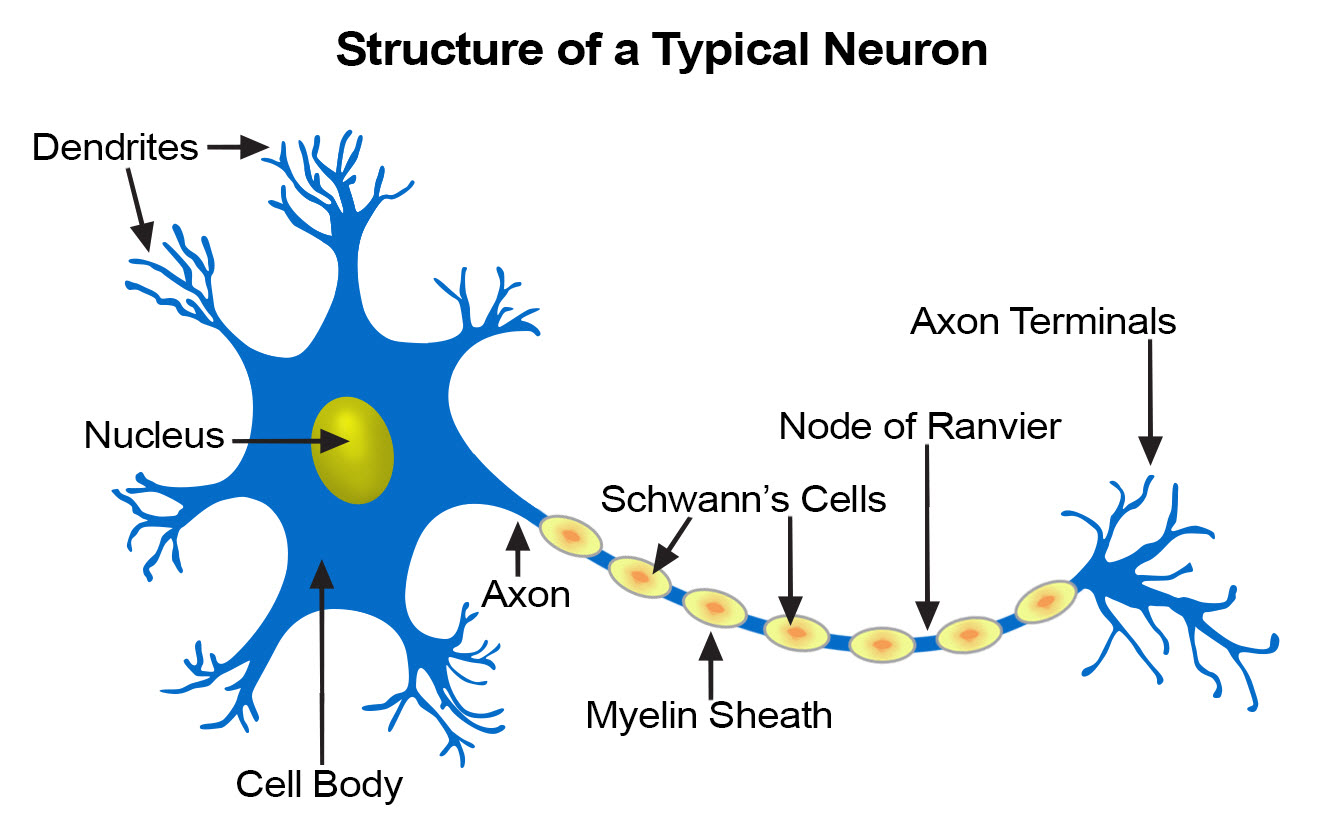
\includegraphics{neuron-structure.jpg}
\end{figure}


Neurons exhibit a membrane potential across their plasma membranes which results form the unequal distribution of electrical charge carried by ions on the two sides of the membrane. When an axon is at rest the value of the membrane potential is called the resting potential. In neurons the resting potential is usually in the range of $-40$ to $-90 mV$. Note that membrane potentials are expressed relative to the extracellular fluid. When the membrane potential is less negative than the resting potential, the cell is said to be depolarized; when it is more negative, the cell is hyperpolarized.

Action potentials are fundamental to a neuron's ability to transfer information; however, there are additional aspects of its electrical properties which shape neuronal input and output. For example, some neurons that fire spontaneously in the absence of external simulation do not fire at regular intervals, but instead generate bursts of action potentials that are separated by the hyperpolarizations of the membrane. Such cells are terms "bursting" neurons \cite{levitan2015neuron}.

These bursts are used in at least two known ways \cite{levitan2015neuron}:

\begin{enumerate}
\item To generate rhythmic behaviors. For example, breathing, walking, swimming, and chewing food.	
\item To secrete neurohormones. Neurohormones are signaling molecules that are released by specialized neurons and transported by the circulatory system to regulate physiology and behavior. For example, neurons located in the hypothalamic region of the mammalian brain individually contain either vasopressin or oxyocin. These hormones control water retention and lactation, respectively. Interestingly, it appears that the bursting pattern is more effective than a steady pacing pattern of firing as a stimulus to the intracellular mechanism which generates peptide release.
\end{enumerate}

\subsection{Mathematical Modeling}

Alan Lloyd Hodgkin and Andrew Huxley, in 1963, won the Nobel Prize in Physiology and Medicine for their work developing the Hodgkin-Huxley (H-H) equations, equations that modeled to incredible accuracy the propagation of action potentials through a squid axon. 

In our project, we seek to capture the important qualitative behaviors of the axon system using electronics. Before speaking of electronics, it is prudent to develop differential equations which simplify the H-H model.

The Hodgkin-Huxley model models the cell membrane as a simple circuit. 

\begin{figure}[h]
    \centering
    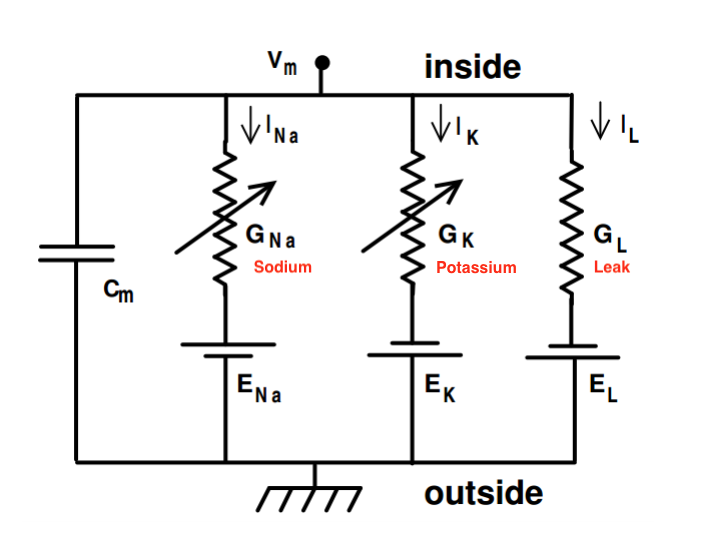
\includegraphics[scale=0.5]{hhmodel}
    \caption{Hodgkin-Huxley Circuit}
    \label{fig:my_label}
\end{figure}

Two voltage-dependent sodium and potassium channels allow the ions to flow through the membrane. The membrane has a capacitance indicated by $c_m$. Additionally, the sodium and potassium channels have a conductance parameter $G_{Na}$ and $G_K$, as well as a leakage conductance as shown. These conductance parameters can be modeled by various functions as will be shown later, and model the buildup in the passage of ions that create the action potential. The circuit is in parallel to mimic the axon. 

Using classic current conservation in a circuit, and adding the parameter $I_{ext}$ of external current, we can derive the current equation for the cell.

\begin{align}
I_{ion} := \sum I_{K} + I_{Na} + I_L \\
    c_m\frac{dV_m}{dt} + I_{ion} = I_{ext}
\label{eq:conduct}
\end{align}

In our particular model, we will assume that $G_L$ is constant and the capacitance $c_m$ as well. $V_m$ is the potential within the cell membrane, and $I_{ion}$ is the net ionic current within the cell.

The derivation of each ionic current through the different channels depends on the conductance parameter times the driving potential.

\begin{align*}
    I_{ion} = G_{ion}(V_{m}-E_{ion})
\end{align*}

where $G_{ion}$ is the conductance of the ionic channels and $E_{ion}$ the corresponding potential.

The physical meaning of conductance is the probability that the channels that the ions pass through will be considered open, or when the gates that the ions can pass through are all permissive in that particular ion channel. This is dependent on the voltage of the cell membrane. 

Define the following differential equation given in terms of $p \equiv p(V, t)$ which is interpreted as a fraction of open gates, and $a(V), b(V)$ which are functions of voltage to be fit empirically. 

\begin{align}
    \frac{dp}{dt} = a(V)(1-p) - b(V)p
    \label{eq:dpdt}
\end{align}

Now, let us consider three separate solutions $p$ to this equation which we term $m, h, n$. 

Hodgkin and Huxley interpreted $m, h, n$ as three different types of gates to model the conductance channels. The conductance $G_{Na}$ and $G_K$ are then modeled as

\begin{align*}
    G_{Na} &= \bar{G}_{Na}m^3h\\
    G_{K} &= \bar{G}_{K}n^4
    \label{eq:gating}
\end{align*}

where $\bar{G}_i$ are constants.

Hodgkin and Huxley discovered that as they kept the voltage constant, the conductance of the channels $m, h, n$ increased steadily to a maximum value. They used this experimental data to achieve equations for the time step of increase of $p$. Note that solutions to the posed differential equation are exponentials given that Equation \ref{eq:dpdt} is first order differential equation linear in $p$. Hence, we can speak of time constants in the usual sense (reaching $1/e$ of the steady state $t \rightarrow \infty$ value).

\begin{align}
    p_{\infty}(V) &= \frac{a_p(V)}{a_p(V) + b_p(V)} \\
    \tau_p(V) &= \frac{1}{a_p(V) + b_p(V)} 
    \label{eq:time}
\end{align}

where $p_{\infty}(V)$ is the steady state value at an given voltage and ${\tau_p}(V)$ are time constants of response of the gates, in relation to $p$ growing to its steady state value. These constants can be experimentally fit to data and using Equation (\ref{eq:dpdt}) we can find $a_p(V)$ and $b_p(V)$. Thus, the final equations for the rate constants are as follows:

\begin{align*}
    a_m(V) &= \frac{0.1(25-V)}{\exp(\frac{25-V}{10})-1}
    &b_m(V) = 4e^{-V/18} \\
    a_n(V) &= \frac{0.01(10-V)}{\exp(\frac{10-V}{10})-1} 
    &b_n(V) = 0.125e^{\frac{-V}{80}}\\
    a_h(V) &= 0.07e^{\frac{-V}{20}} 
    &b_h(V) = \frac{1}{\frac{\exp(30-V)}{10}+1}
\end{align*}

We can also rewrite equation (\ref{eq:dpdt}) as the following

\begin{align*}
    \frac{dp}{dt} = \frac{p_{\infty}(V)-p}{\tau_p(V)}
\end{align*}

The combined system of differential equations is shown in the next section. Furthermore, in Figure \ref{fig:inf} we show the values of $m_\infty$ and $n_\infty$ derived using the equations above. 

\begin{figure}[h]
\centering
	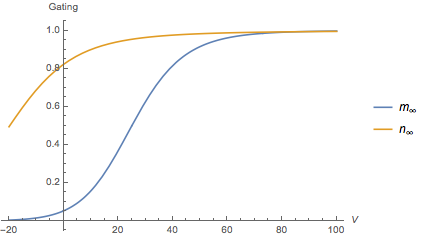
\includegraphics[height=5cm]{gating.png}
	\caption{f$m_{\infty}$ (blue) and $n_{\infty}$ (orange)}
		\label{fig:inf}
\end{figure}

\subsection{Circuit Modeling} 

Maeda and Makino \cite{maeda2000pulse} show how to model a neuron using 3 transistors for a FitzHugh-Nagumo type neuron. In the FitzHugh-Nagumo model, one simplifies the Hodgkin-Huxley formulation by replacing the fast Na current of the H-H model with a simplified fast, depolarizing, activation process. Furthermore, one replaces the slow $Na$ inactivation and slow, repolarizing, $K$ current by a single slow inactivation process. By adding one more repolarizing process, modeled by two more transistors, they can produce a neuron with bursting behavior. 

The state variables for the model are $V$, $m$, $h$, and $n$ defined by Equation \ref{eq:dpdt} as before. Hence, we can combine Equations \ref{eq:conduct} and \ref{eq:gating}.

\begin{align*}
    C\frac{dV}{dt} &= I_{ext} -\bar{G}_{Na}m^3h(V-E_{Na}) -\bar{G}_{K}n^4(V-E_{K})  -\bar{G}_{L}m^3h(V-E_{L}) \\
    \frac{dm}{dt} &= \frac{m_{\infty}(V)-m}{\tau_m(V)} \\
    \frac{dh}{dt} &= \frac{h_{\infty}(V)-h}{\tau_h(V)} \\
    \frac{dn}{dt} &= \frac{n_{\infty}(V)-n}{\tau_n(V)} 
\end{align*}

While analyzing a four-dimensional nonlinear system is certainly feasible, it is difficult to then visualize our results. Furthermore, the number of combinations of parameters grows exponentially with each new parameter introduced. Hence, we seek to reduce the model complexity.

\begin{figure}[h]
\centering
\begin{subfigure}{.5\textwidth}
	\centering
	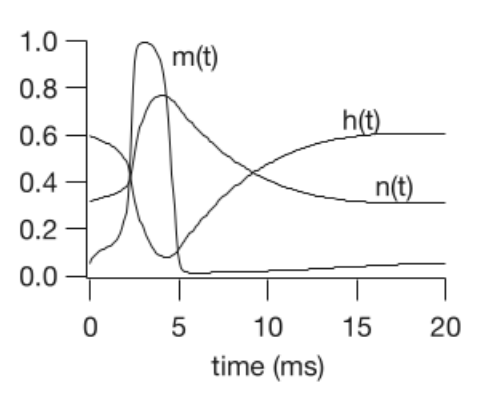
\includegraphics[height=5cm]{keener1.png}
	\caption{Gate Variables. From equation \ref{eq:gating} we see that this diagram depicts evolution in conductance of the circuit for each gate, up to a constant factor.}
\end{subfigure}%
\begin{subfigure}{.5\textwidth}
	\centering
	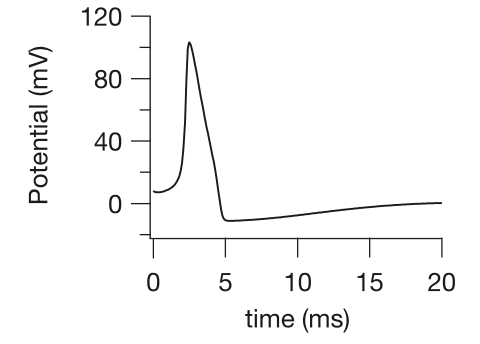
\includegraphics[height=5cm]{keener2.png}
	\caption{Action Potential. We can see the connection with Figure \ref{fig:action-explained}. For example, after the discharge we see a "knee" which extends below the rest potential.}
\end{subfigure}
	\caption{Dynamics of H-H model Without Approximation on Shared Time-Scale (ms)}
	\label{fig:keen}
\end{figure}


From Equation \ref{eq:time}, it's clear that the time constants, $\tau_i$ vary widely between these equations. For example, for a 20 mV potential, the values are $\tau_m \approx 0.4 ms$, $\tau_h \approx 8 ms$, and $\tau_n \approx 5 ms$. In general, it is true that $\tau_m$ is much smaller than the other time constants. Recall that $\tau_m$ is a measure of the speed with which $m$ converges to its steady state value $m_\infty$. Therefore, it may be a reasonable assumption to assume that $\tau_m$ is so fast compared to the other parameters that $m = m_\infty$. Then, we can either take $n$ or $h$ to be constant which would then give us a two-dimensional nonlinear system. Since $h$ fluctuates over the largest time-scale, we'll take it to be some constant $\bar{h}$. As a result, we have 

\begin{align*}
        C\frac{dV}{dt} &= I_{ext} -\bar{G}_{Na}m_\infty^3\bar{h}(V-E_{Na}) -\bar{G}_{K}n^4(V-E_{K})  -\bar{G}_{L}(V-E_{L}) \\
    \frac{dn}{dt} &= \frac{n_{\infty}-n}{\tau_n} 
\end{align*}

The assumption of taking $h$ to be constant can be judged visually in Figure \ref{fig:keen}, borrowed from Keener and Sneyd, which shows values of the unapproximated model\cite{keener}. Indeed, the neurons we construct in this project follow from this approximation.

\section{Circuit 1: A Pulse Type Neuron}
\label{sec:pulse-neuron}

\subsection{Theory}
 
 We begin by considering a circuit with the following structure
 
\begin{figure}[H]
\centering
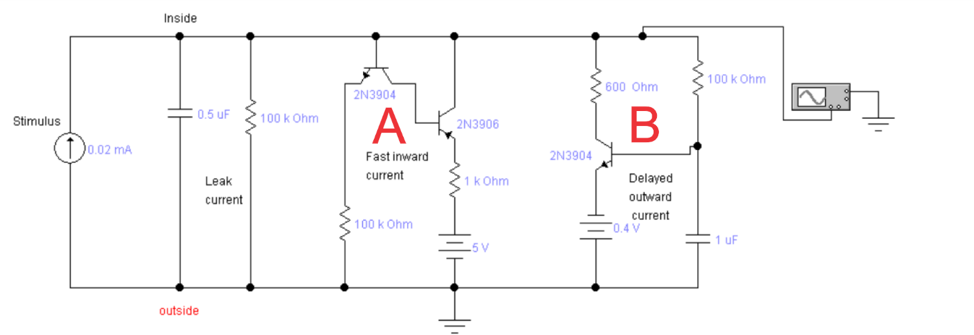
\includegraphics[width=0.8\textwidth]{exercise1-0}
\caption{"A pulse type neuron model" from \cite{maeda2000pulse}}
\label{fig:maeda-pulse}
\end{figure}

In our experiment, instead of applying a constant current source we added a $200k\Omega$ resistor above the $5V$ voltage source. Nevertheless, the analysis follows similarly.

Hence, we consider transistor sub-circuits $A$ and $B$ as ideal switches. When we just turn on the current source, the upper node voltage is equal to 0. Because both switches are off, the circuit can be reduced to the following circuit:
 
\begin{figure}[H]
\centering
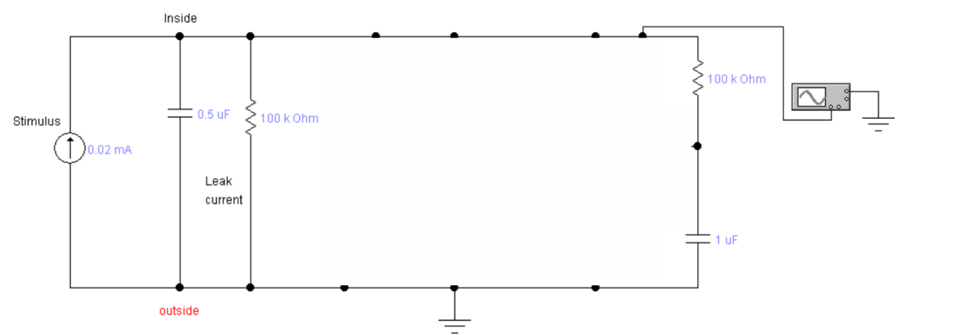
\includegraphics[width=0.8\textwidth]{exercise1-1}
\end{figure}

The dynamic of the upper node $V(t)$ depends on the values of capacitors and resistors, but the final (equilibrium) voltage depends only on the stimulus current $I$ and leak current resistor. If we are not interested in dynamics of $V(t)$, but only in its equilibrium value, we can remove capacitors from the circuit.
 
\begin{figure}[H]
\centering
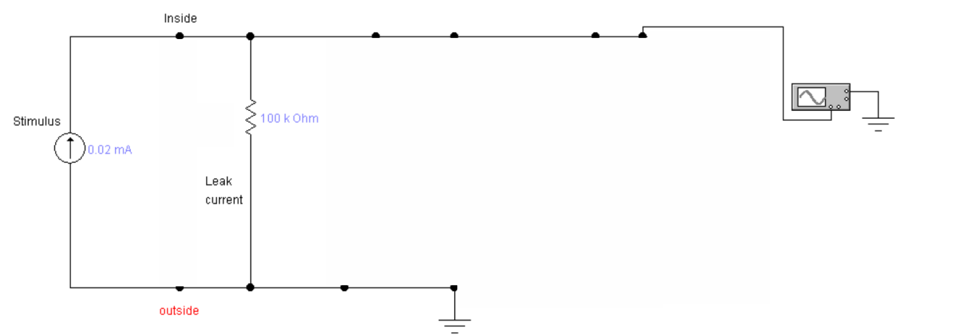
\includegraphics[width=0.8\textwidth]{exercise1-2}
\end{figure}

Clearly, we have

\begin{align*}
(100k\Omega)(0.02 mA) = 	2V
\end{align*}

Now, let's turn on switch $A$
 
 \begin{figure}[H]
 \centering
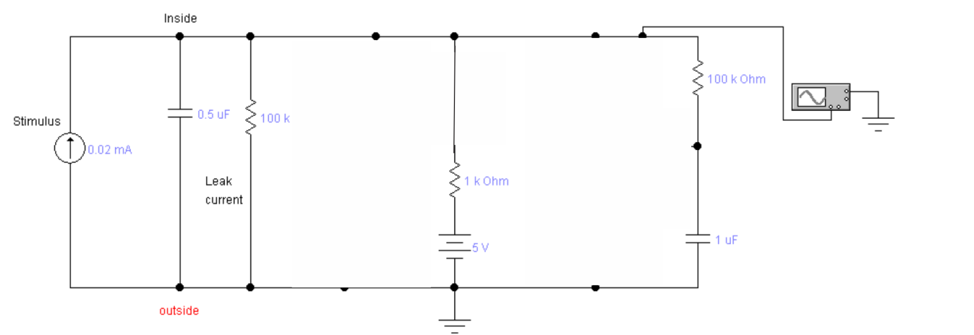
\includegraphics[width=0.8\textwidth]{exercise1-3}
\end{figure}

If we again are not interested in dynamics of $V(t)$, we can redraw the circuit dropping all capacitors
 
 \begin{figure}[H]
 \centering
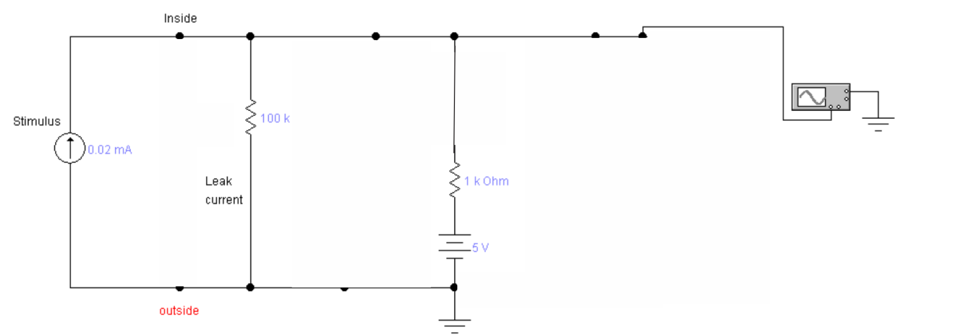
\includegraphics[width=0.8\textwidth]{exercise1-4}
\end{figure}

To find the voltage at the top node, we simply use the method of Thevenin's equivalent circuit\cite{fortney1987principles}. To calculate the Thevenin equivalent voltage, we may open all current sources and calculate the voltage at the top node. In which case, we find that we have a voltage divider which gives 

$$\frac{100}{1+100} * 5V = 4.95 V$$

Now, let's turn on the switch $B$
 
 \begin{figure}[h]
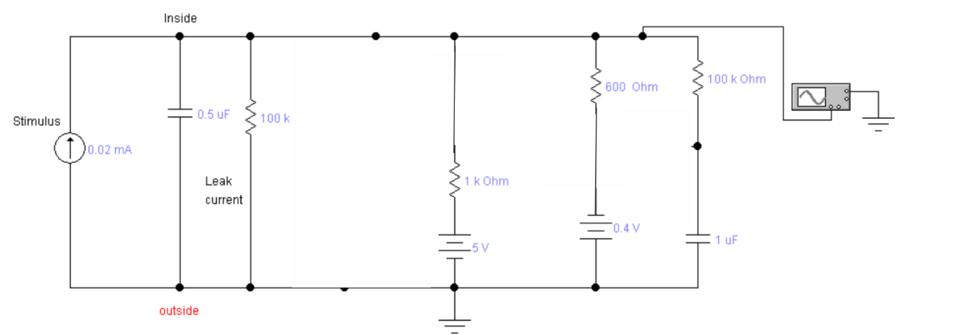
\includegraphics[width=0.8\textwidth]{exercise1-5}
\end{figure}

and drop all capacitors again
 
\begin{figure}[H]
\centering
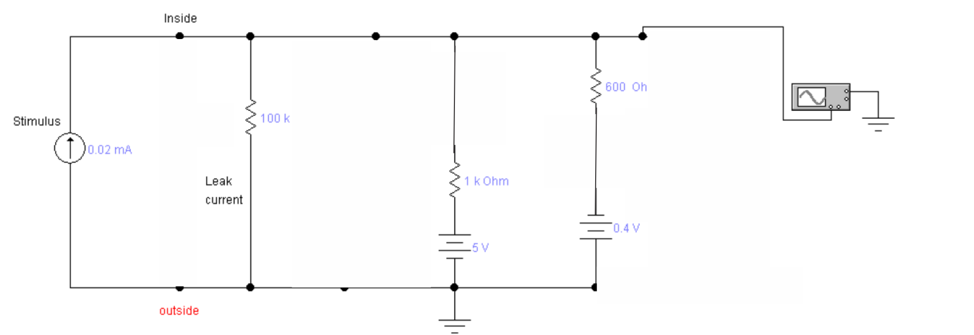
\includegraphics[width=0.8\textwidth]{exercise1-6}
\end{figure}

We can use the method of Norton, first computing $R_{N}$ by shorting all voltage sources and opening all current sources. Then, we have three resistors in parallel with $R_{N} = 373 \Omega$. Next, we compute $I_N$ by adding a short wire between the top and bottom node. This then gives current $I_N = 0.02 mA + 5 mA - 0.4/0.6 mA = 4.35 mA$. Hence, we have $V_{Th} = 1.6 V$.

Therefore, by modeling our circuit in terms of changes in voltage equilibria induced by which transistors are open (viewing transistors as ideal switches), we have located three different steady states. The dynamic which determines the rate at which the circuit evolves towards the particular equilibrium dictated by the open switches is determined by the capacitance values because these define the time constants of the resistor-capacitor subcircuits (of course resistance can be changed to move the time constant as well). Finally, the transition between which switches are open depend on the characteristics of the transistors (e.g. NPN vs. PNP and $\alpha, \beta$).

In the context of our circuit, we can then describe the expected behavior visually below.

\begin{figure}	
\label{fig:action-explained}
\end{figure}
 

\subsection{Results and Discussion}

We constructed the circuit faithfully in accordance with Figure \ref{fig:maeda-pulse}, finding no need for modification\footnote{However, recall that instead of applying a constant current source, we added a $200k\Omega$ resistor above the $5V$ voltage source.}. Our circuit exhibited the expected pattern of an action potential in  a pulse type neuron.

\begin{figure}[h]
\centering
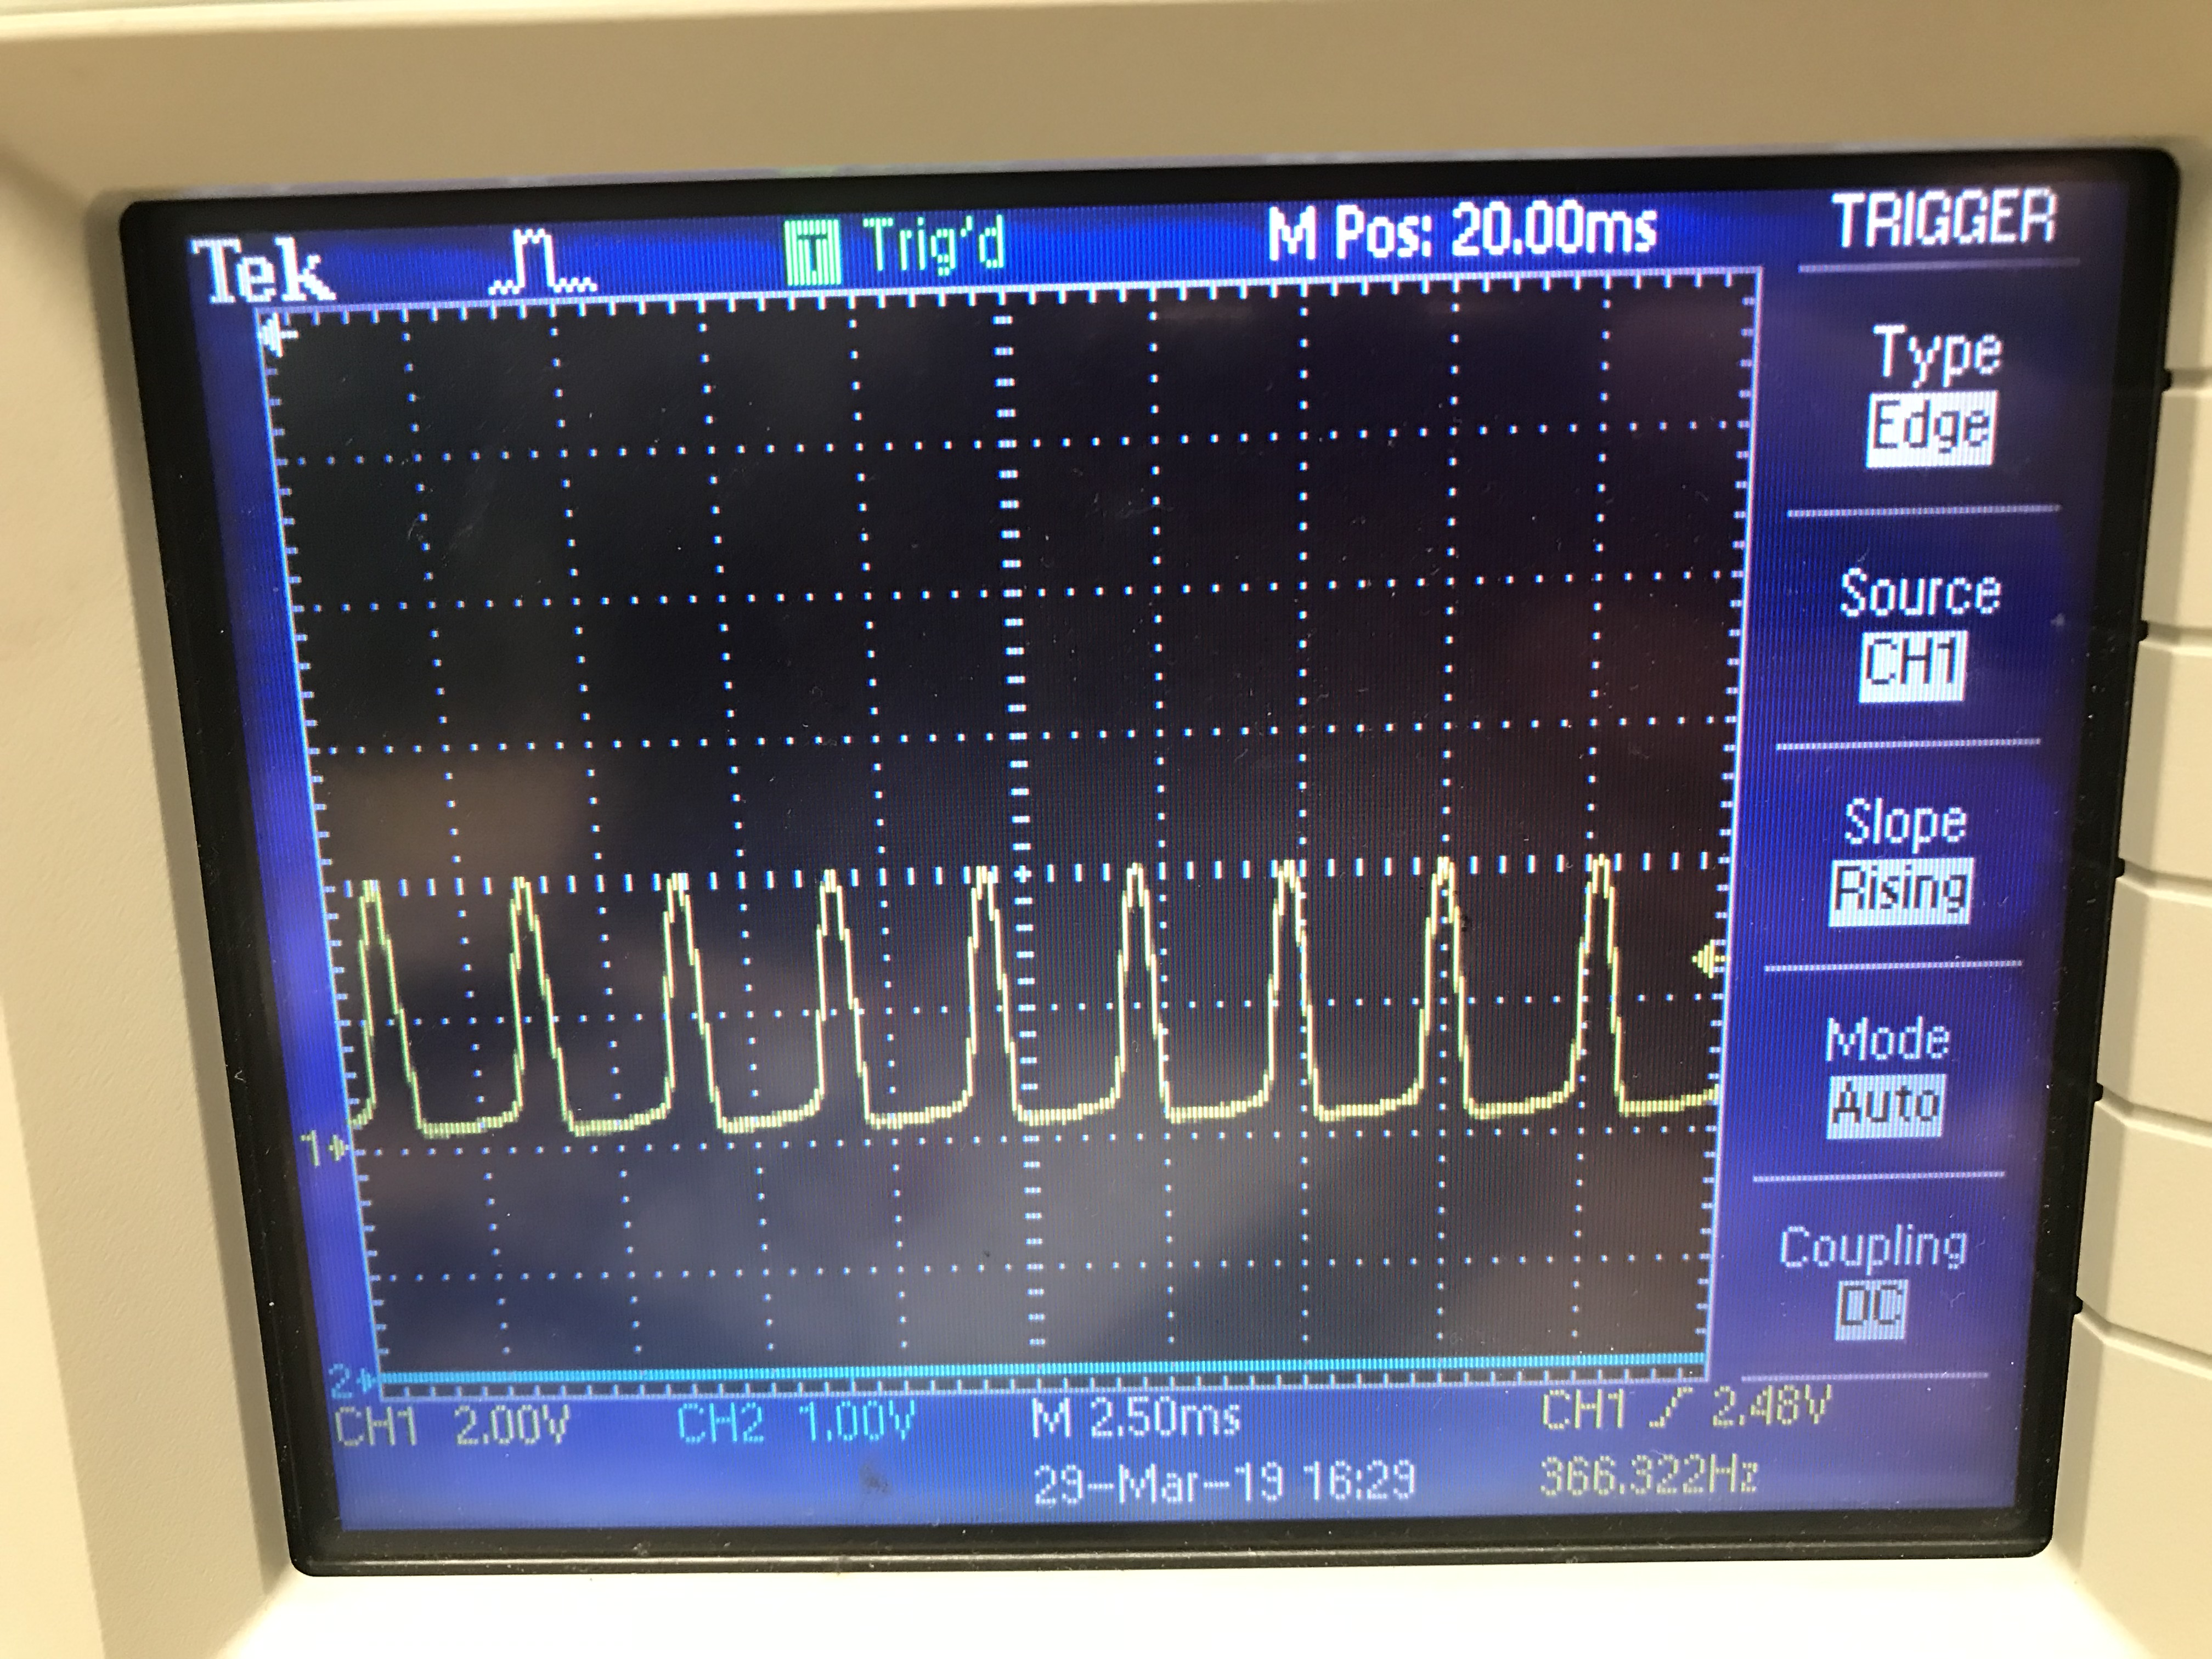
\includegraphics[width=0.7\textwidth]{neuron.jpeg}	
\caption{Oscilloscope for Pulse Type Neuron}
\label{fig:pulse}
\end{figure}

From the Figure \ref{fig:pulse}, we see that the slow repolarization current (associated with the charging of the $0.5 \mu F$ capacitor) increases the voltage just short of $1 V$ before the fast current opens, falling short of the $2V$ equilibrium theoretical prediction. This is because the transistor which opens the fast current ($A$) is opened before this equilibrium can be reached.

Furthermore, we see that the action potential reaches its maximum at approximately $4 V$, falling short of the theoretical prediction of $4.95V$. This likely indicates that the depolarizing current is activated from switch $B$ before the $1 \mu F$ capacitor is fully charged. Nevertheless, we do not wish to reduce this time constant because we would then activate the fast current prematurely so as to subsume the slow current.

We see that we have captured the essential details of the mathematical action potential shown in Figure \ref{fig:keen}. For example, looking closely, we see the "knee" after the discharge face which extends the potential below the rest potential before returning back to equilibrium. 

\section{Circuit 2: A Pulse Type Neuron with Burst}

\subsection{Theory}

\begin{figure}[h]
\centering
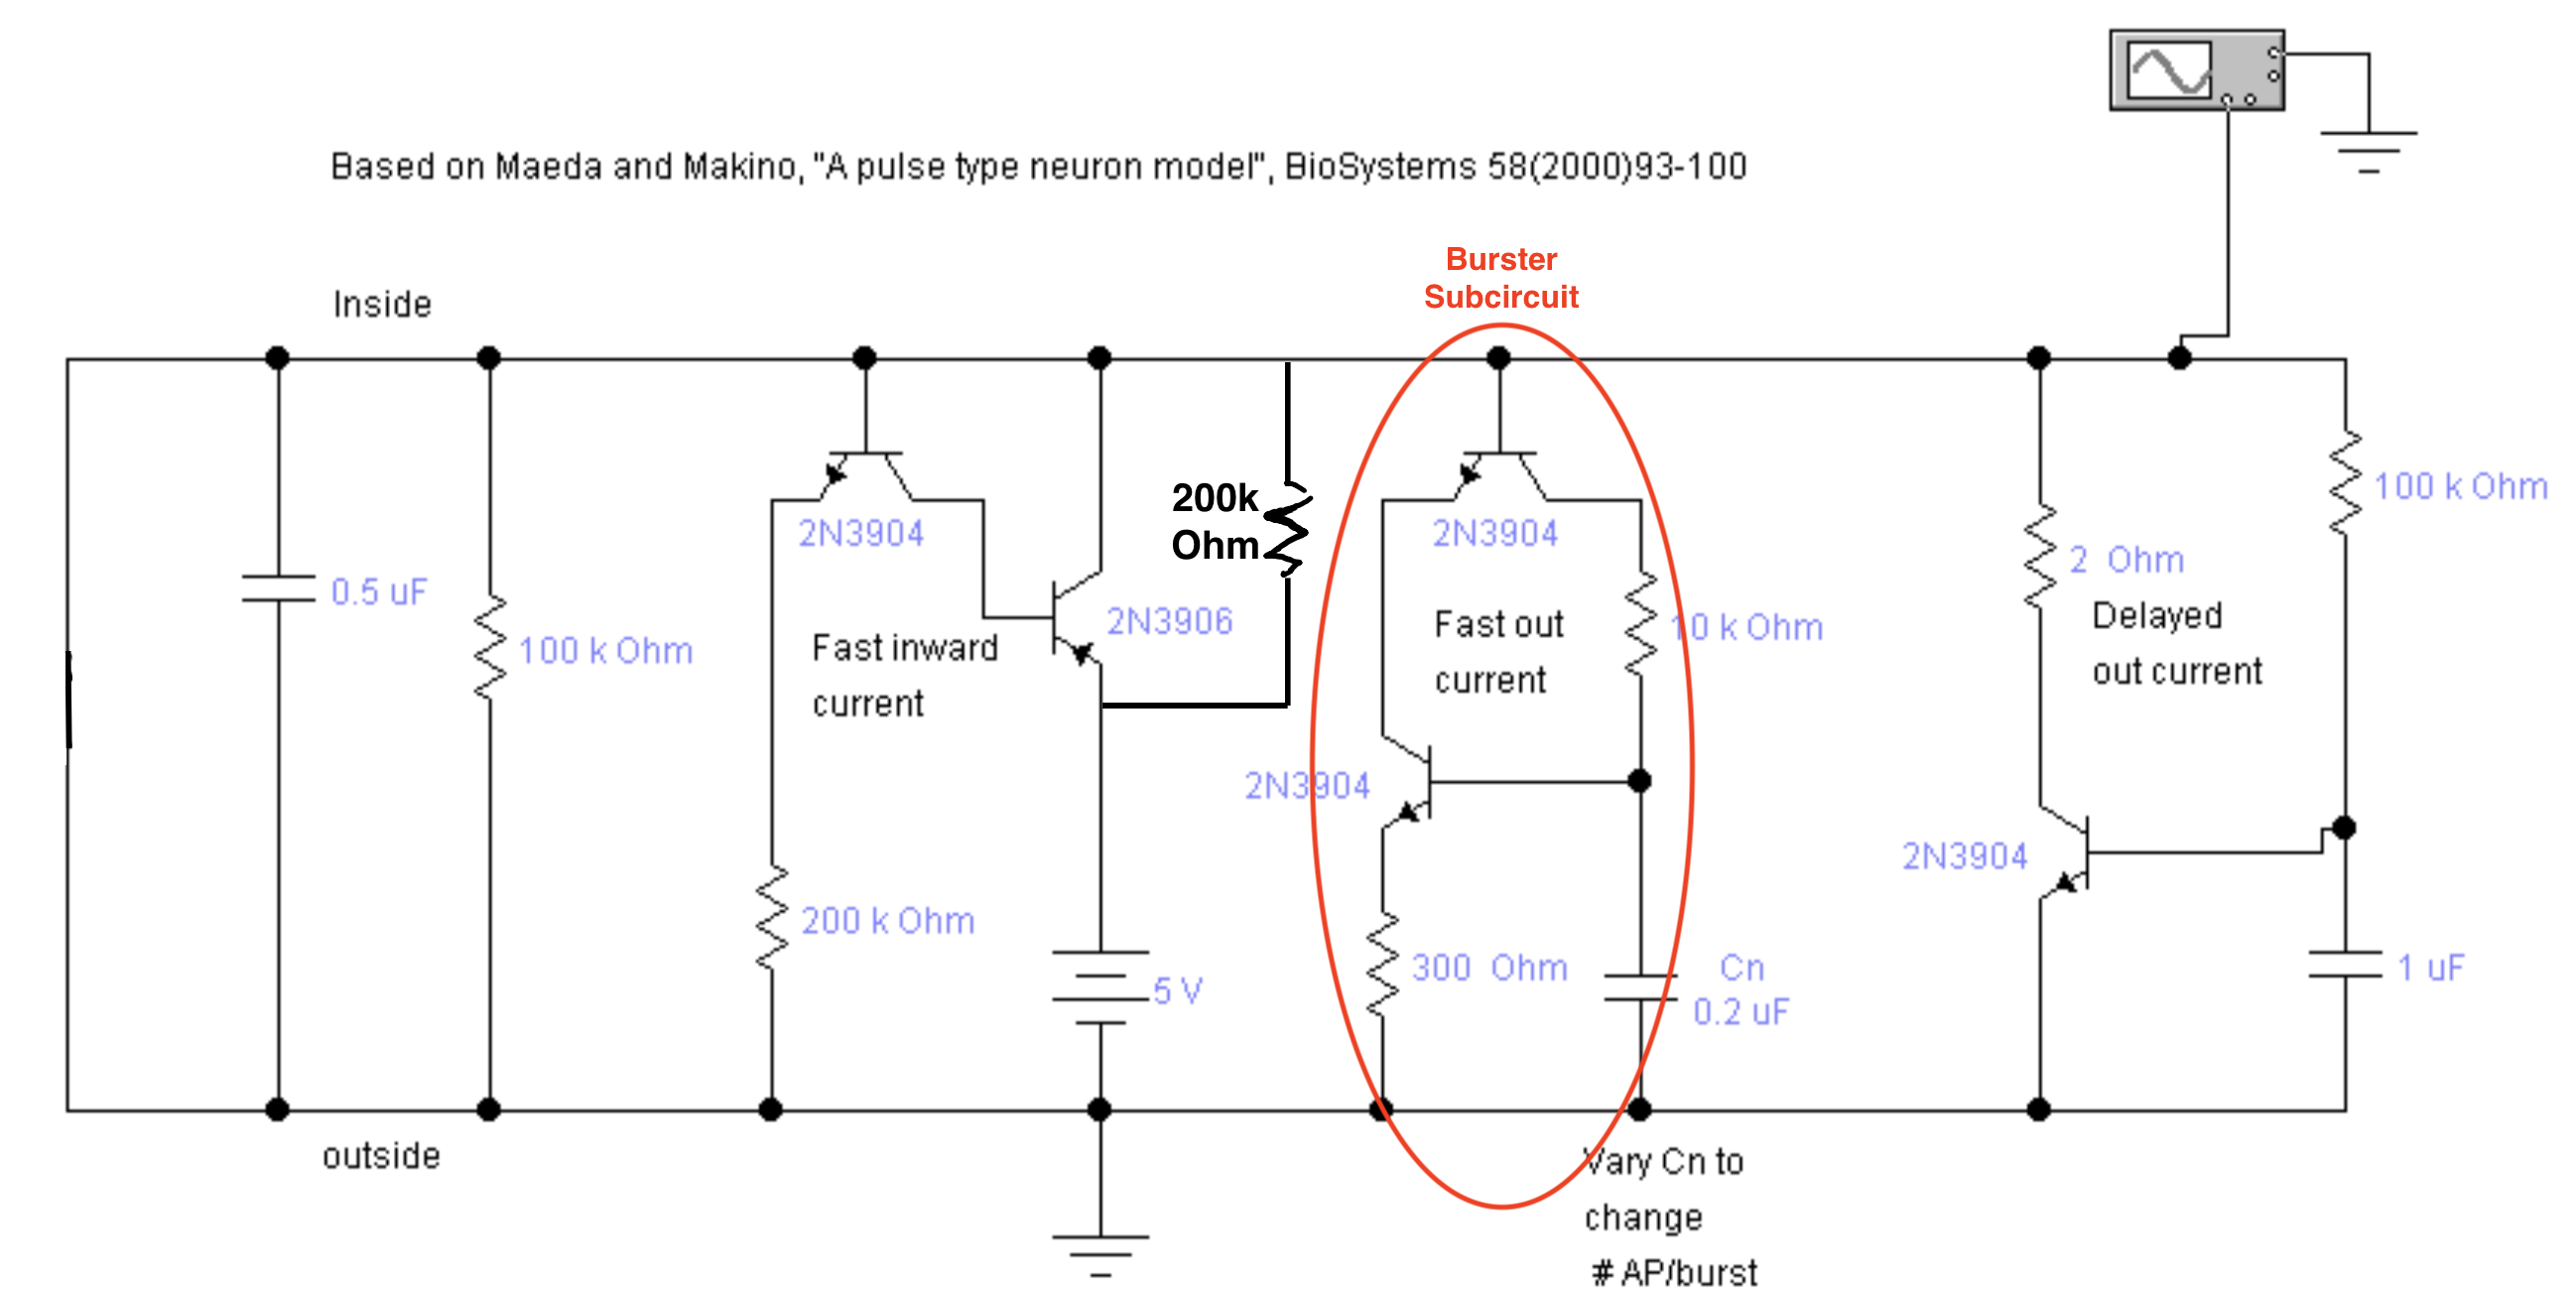
\includegraphics[width=\textwidth]{burster_heart_cell}	
\caption{Burster Heart Cell}
\end{figure}

The primary modification created for this circuit as opposed to the pulse type is a burster component (the subcircuit who intersects with the top node at the third dotted intersection from the right). When the top node reaches sufficient voltage, the top transistor of this subcircuit is opened. Then, the second transistor opens after a time dictated by the time constant associated with the capacitor within this subcircuit. Hence, the fast current can flow out through the $300 \Omega$ resistor. Nevertheless, after enough voltage has been drained the top transistor closes and the fast current begins to recharge the top node again, repeating the process. This creates the bursts we hope to model.

Throughout this process the $1 \mu F$ capacitor continues to charge because the frequency of bursts is below the cutoff frequency defined by $R = 10k \Omega, C = 0.2 \mu F$ (approximately $1/RC = 200 Hz$). Hence, once this capacitor charges and the adjacent transistor opens voltage rapidly drains through the $2 \Omega$ resistor resulting in the depolarization of the action potential, per usual. One comparison to note with the pulse type circuit is that this $2 \Omega$ resistor was $600 \Omega$ in the previous circuit. Hence, we expect a steeper, near-instantaneous drain at the end of the action potential. Furthermore, the fast inward current path previously had a $1k \Omega$ resistor which is now simply a short in this circuit. Hence, "fast" charging occurs theoretically instantaneously in this circuit.

Referring back to Figure \ref{fig:action-explained}, we expect the fast charge and fast discharge to appear as a rectangular "window". This then allows for the top transistor of the burster circuit to open and close in close temporal proximity to the fast charge and discharge, creating a window for bursting.

\subsection{Results and Discussion}

We constructed the circuit faithfully in accordance with Figure \ref{fig:maeda-burst}, finding no need for modification.

\begin{figure}[h]
\centering
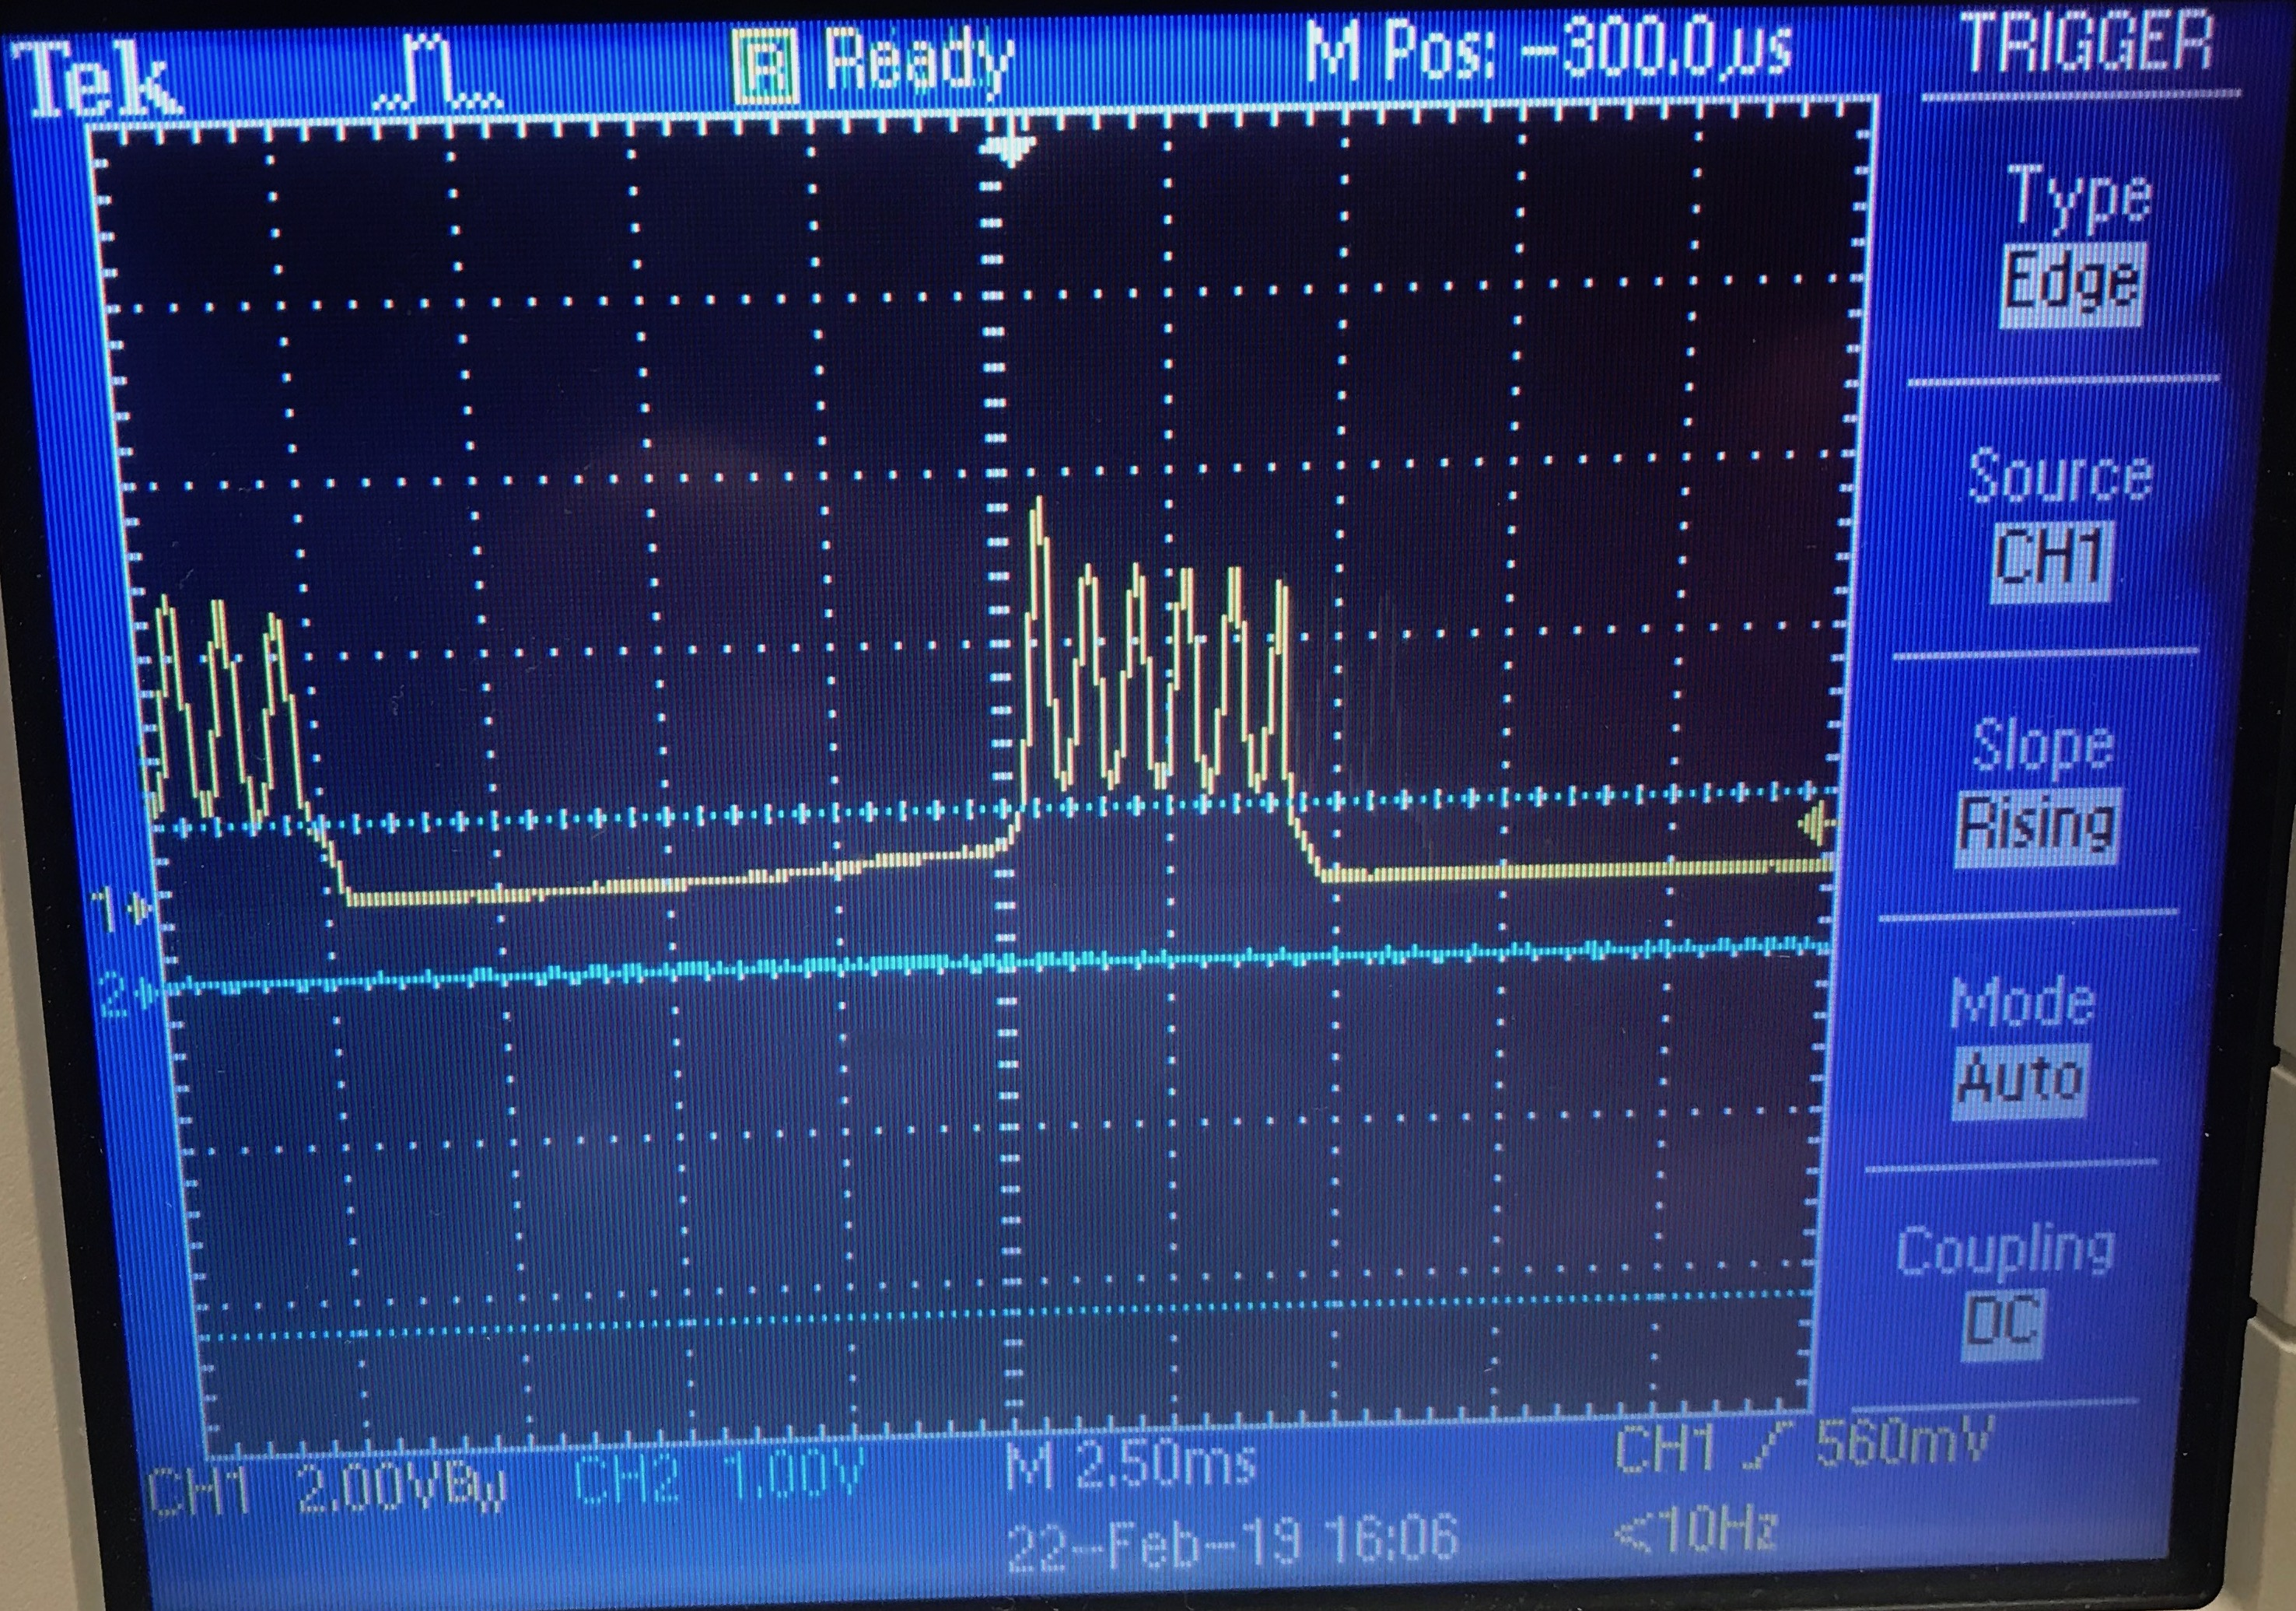
\includegraphics[width=0.7\textwidth]{burster_osc}
\caption{Oscilloscope for Burst Neuron}
\label{fig:maeda-burst}
\end{figure}

As anticipated, we see the usual action potential magnitudes associated with the pulse type neuron ($4V$ maximum, $1V$ for the slow charge peak). However, we also see oscillatory "bursting" behavior during the fast charge phase.

\chapter{Synapses}

\section{Introduction}

\subsection{Overview}

Information transfer from one part of the nervous system to another involves a highly specialized structure of the neuron known as the synapse. There exist two types of synapses: chemical synapses and electrical synapses. 

Electrical synapses allow direct, passive flow of electric current through special intercellular connections called gap junctions. These gap junctions allow for virtually instantaneous transmission of electrical signals through direct passive flow of ions between neurons. The main goal of electrical synapses is to synchronize electrical activity among populations of neurons. 

Chemical synaptic transmission is the transfer of neurotransmitters or neuropeptides from a presynaptic axon to a postsynaptic dendrite. Unlike an electrical synapse, the chemical synapses are separated by a space called the synaptic cleft.

A presynaptic neuron may increase the probability of an action potential occurring in a postsynaptic cell. This is known as an excitatory postsynaptic potential (EPSP). It most commonly occurs via the vesicular release of neurotransmitters (most commonly glutamate) from the presynaptic axon terminal into the synaptic cleft, as in a chemical synapse.

On the opposite end, neurotransmitters such as GABA can cause hyper-polarization in the postsynaptic cell, a phenomenon known as an inhibitory postsynaptic potential (IPSP).

\section{Circuit 1: Excitatory Synapse}

\subsection{Theory}

\begin{figure}[h]
\centering
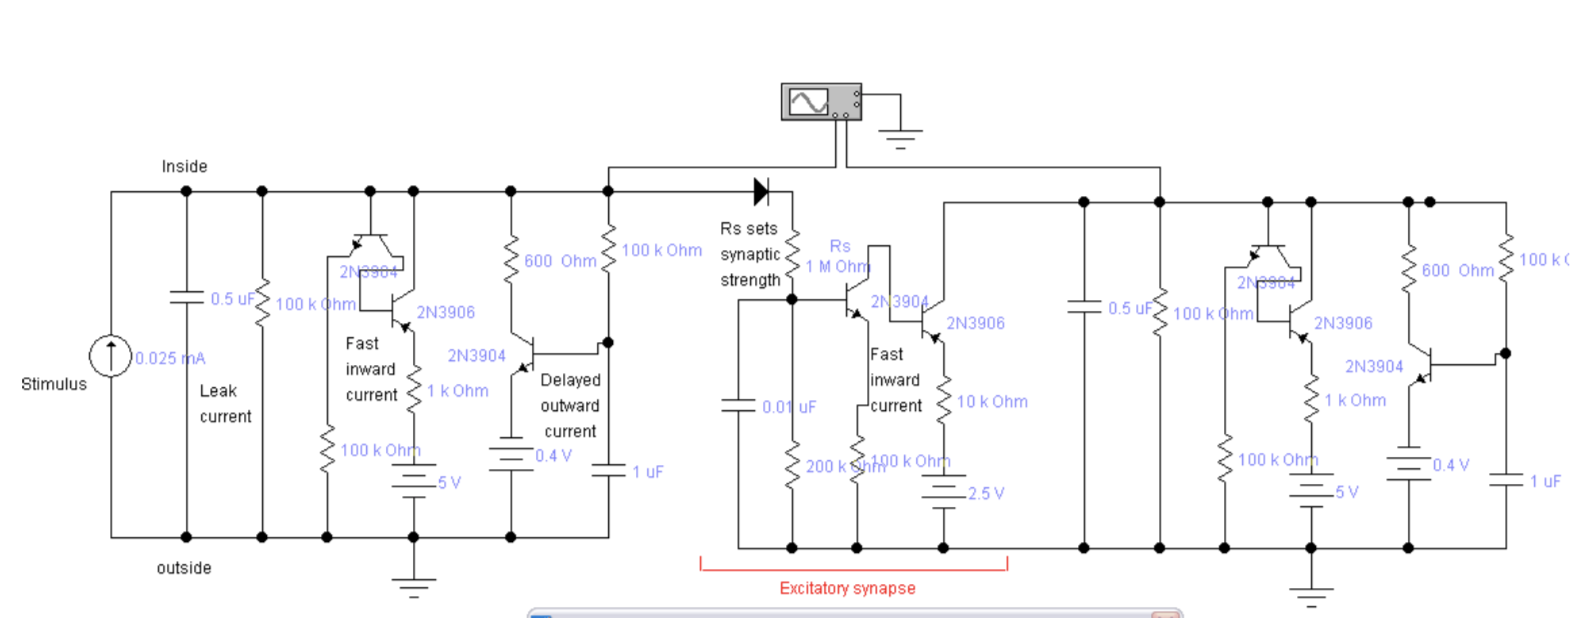
\includegraphics[width=\textwidth]{excitatory_circuit}	
\caption{EPSP Circuit from \cite{levitan2015neuron}}
\label{fig:epsp}
\end{figure}

As usual, instead of applying a constant current source, we added a $200k\Omega$ resistor above the $5V$ voltage source.

In the circuit diagram above (\ref{fig:epsp}), we have two pulse type neurons from the first chapter connected by a synapse subcircuit. However, we have the important modification that a current source only exists within the presynaptic cell. A diode is utilized so that current flows in a single direction, from a presynaptic cell to a postsynaptic one.  

When the current on the top node of the synapse reaches sufficient voltage, the synapse's transistors open. This then allows current to flow out into the postsynaptic cell due to the $2.5V$ source in the synapse. We see that the voltage on the top node has dynamics described by the RC circuit with $R=200 k \Omega, C = 0.01 \mu F$. Hence, this dynamic allows for action potentials to not be excited in the postsynaptic cell for every action potential within the presynaptic cell given that the time constant for the RC circuit is sufficiently great compared to the frequency of action potentials. When current flows into the postsynaptic cell, it reduces the voltage on the top node of the synapse closing the transistors thereby restarting the charging of the capacitor for the RC circuit.

\subsection{Results and Discussion}

\begin{figure}[h]
\centering
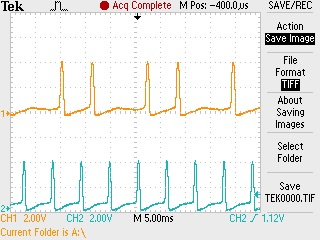
\includegraphics[width=0.7\textwidth]{excitatory.jpg}
\caption{Oscilloscope for Excitatory Synapse}
\end{figure}

In order to see the expected behavior we had to modify the resistor to be $200 \Omega$ from $1 M \Omega$. This significantly increases the "synaptic strength" so as to allow more current to flow towards the postsynaptic cell. In particular, this change directly allows for more current to flow through the synapse transistor base allowing it to open more frequently and rapidly, thereby allowing the potential within the synapse to transfer more signal to the postsynaptic cell. This was necessary because previously the postsynaptic cell exhibited no action potentials before the change.

After this change, we then see that the action potentials of the presynaptic cell (blue), which has a current source, are able to generate action potentials in the postsynaptic cell (yellow) which does not have a current source.  

The magnitude of the action potential remained roughly $4V$ as for the pulse type neurons of the first chapter and similarly for the slow charge and depolarization magnitudes.

\section{Circuit 2: Inhibitory Synapse}

\subsection{Theory}

\begin{figure}[h]
\centering
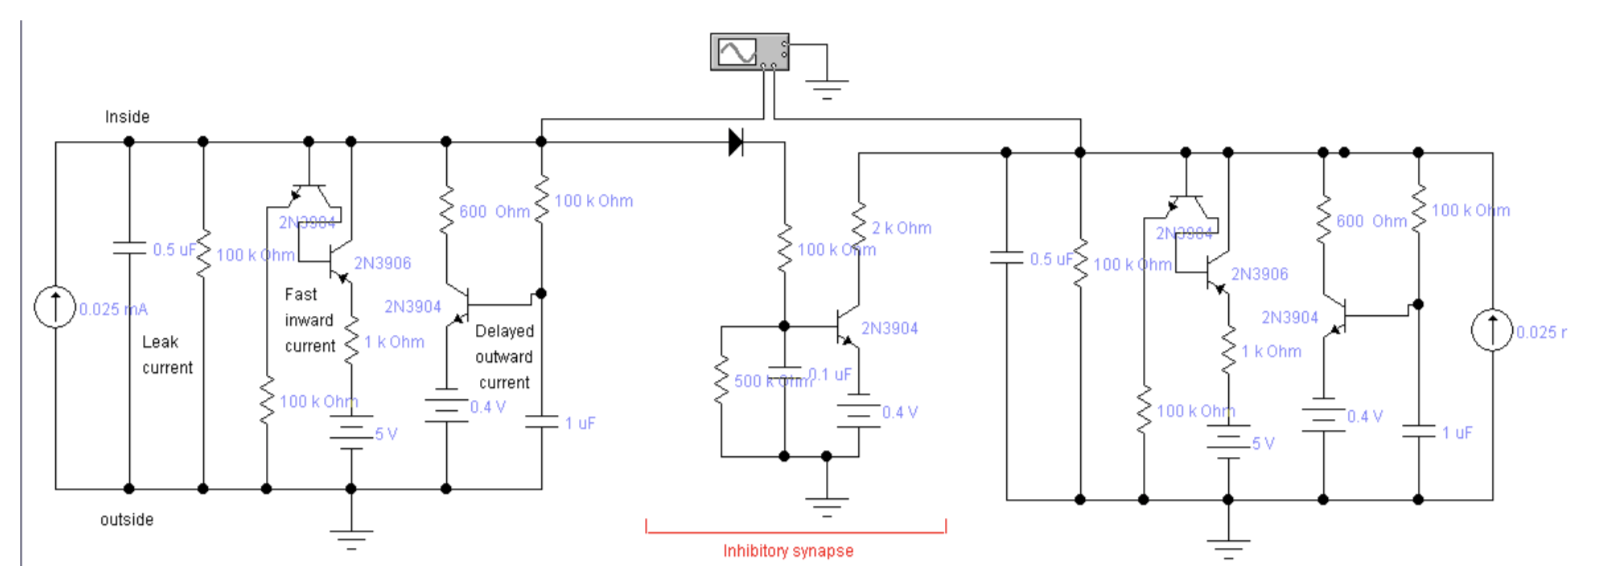
\includegraphics[width=\textwidth]{inhibitory_circuit}	
\caption{IPSP Circuit from \cite{levitan2015neuron}}
\label{fig:ipsp}
\end{figure}

As usual, instead of applying a constant current source, we added a $200k\Omega$ resistor above the $5V$ voltage source.

The diagram (\ref{fig:ipsp}) shows two pulse type neurons from the first chapter connected by a synapse subcircuit. A diode is utilized so that current flows in a single direction, from a presynaptic cell to a postsynaptic one. When the current on the top node of the synapse reaches sufficient voltage, the synapse's transistor opens. This then allows current to flow out of the postsynaptic cell due to the $-0.4V$ source in the synapse. We see that the voltage on the top node has dynamics described by the RC circuit with $R=500 k \Omega, C = 0.1 \mu F$. Hence, this dynamic allows for action potentials to not be inhibited completely in the postsynaptic cell given that the time constant for the RC circuit is sufficiently great compared to the frequency of action potentials. When current flows from the postsynaptic cell into the synapse it reduces the voltage on the top node thereby restarting the charging of the capacitor for the RC circuit.

\subsection{Results and Discussion}

\begin{figure}[h]
\centering
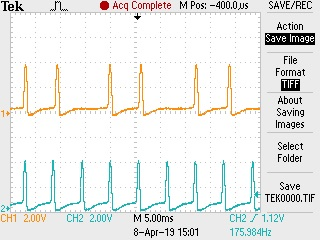
\includegraphics[width=0.7\textwidth]{inhibitory.jpg}	
\caption{Oscilloscope for Inhibitory Synapse}
\end{figure}

In order to see the expected behavior we had to modify the resistor which flows out of the synapse towards the postsynaptic cell to be $39k \Omega$ from $2k \Omega$. This decreases the "synaptic strength" so as to reduce the current which damps the postsynaptic cell. This was necessary because previously the postsynaptic cell exhibited no action potentials. For the same reason, we reduced the damping voltage within the synapse to be $0.2 V$. 

Furthermore, we tuned the $0.4 V$ voltage source within each cell to be $0.36 V$ which reduces depolarization for each of the cells. 

After this change, we then see that the action potentials of the presynaptic cell (blue), which has a current source, occasionally prevent action potentials in the postsynaptic cell (yellow) which also has a current source, as expected. When the synapse is disconnected, the cells fire similarly each exhibiting regular action potentials, also as expected.

The magnitude of the action potential remained roughly $4V$ as for the pulse type neurons of the first chapter and similarly for the slow charge and depolarization magnitudes. 
\chapter{Central Pattern Generators}

\section{Introduction}

\subsection{Overview}

The goal of the circuit in this chapter is to connect two neuron cells in a way such that they fire out of phase with one another.

Many animal behaviors, such as walking or swimming, require the rhythmic contraction of muscles. Most rhythmic behaviors require that opposing groups of muscles be contracted and relaxed in a coordinated manner and so requiring the coordination of a network of neurons.

The very simplest circuit that can generate alternating contraction and relaxation in two different muscles consists of only two neurons. Each neurons makes an inhibitory synapse with the other. For this behavior to exist, it is necessary that after the membrane potential of the cell has been hyper-polarized for a short period of time, the cell becomes more excitable than usual. When the membrane is then allowed to return toward its normal resting potential, one or more action potentials may result. This behavior is known as "post-inhibitory rebound" Some explanations for such behavior include inward current such as a voltage-dependent sodium current or a nonselective cation current called the H-current.

An action potential in an upswing neuron generates an inhibitory postsynaptic potential (IPSP) in a downswing neuron. Because of post-inhibitory rebound, the downswing neuron generates an action potential at the end of the IPSP. This in turn triggers an IPSP in the upswing neuron. This upswing neuron then fires faster than the next approaching action potential of the other neuron as a result of inhibitory rebound; hence, this neuron can send signal to the synapse rapidly enough to create the response that shorts the other neuron.

\begin{figure}[h]
\centering
\includegraphics[width=0.7\textwidth]{ipsp.png}	
\caption{p. 461 of \cite{levitan2015neuron}}
\end{figure}

\section{Circuit: Inhibitory Pattern Generation}

\subsection{Theory}

\begin{figure}[h]
\centering
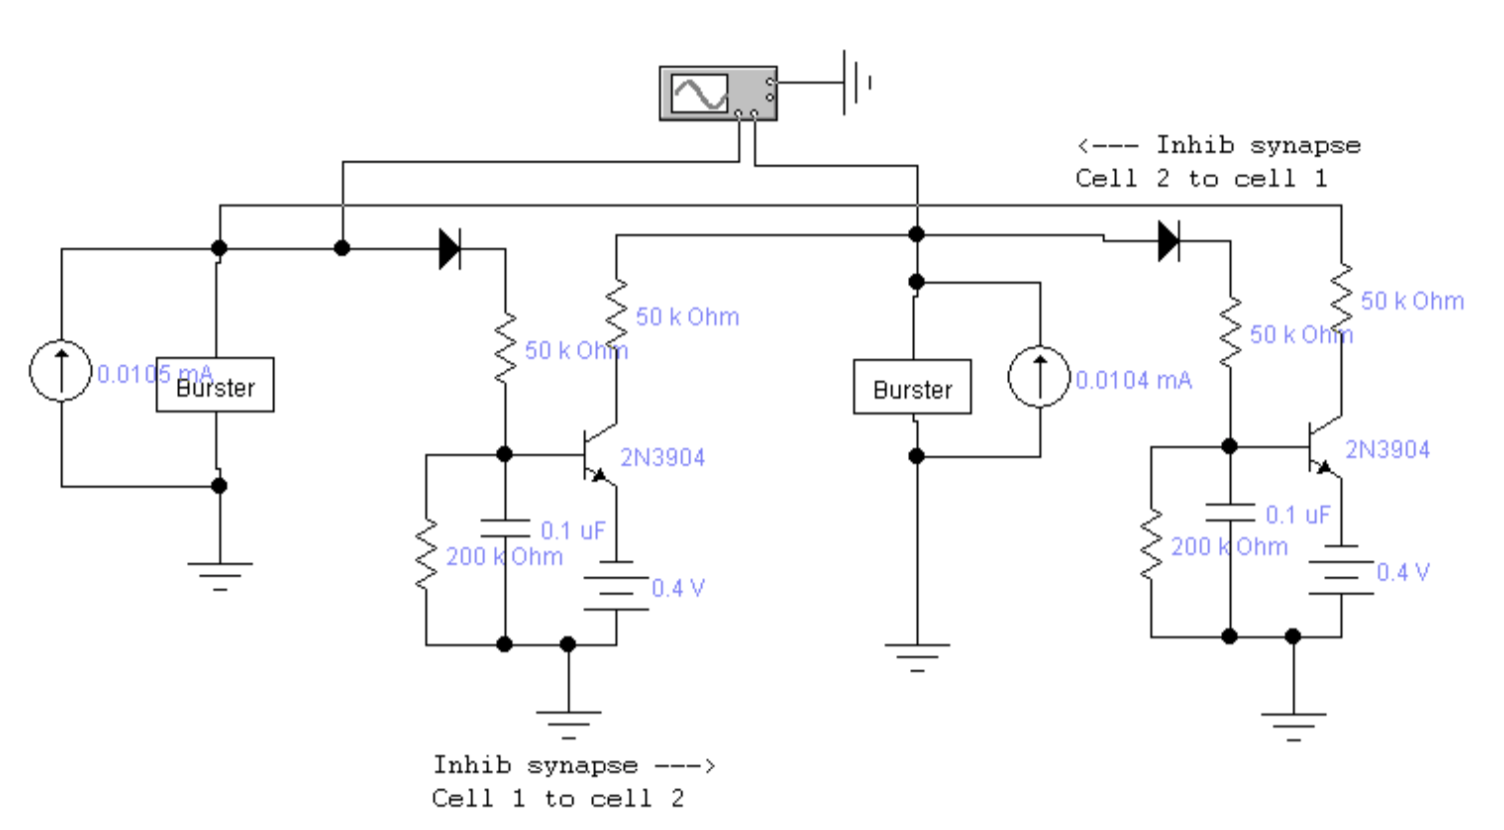
\includegraphics[width=\textwidth]{pattern_circuit}	
\caption{Alternate Bursting Circuit from \cite{maeda2000pulse}}
\label{fig:pattern}
\end{figure}

Here, we consider the circuit in Figure \ref{fig:pattern}. However, instead of using burster cells (as they are depicted in the figure), we use ordinary neuronal cells as in Section \ref{sec:pulse-neuron}.

In the previous chapter, we saw a circuit with a single diode driving current from one neuronal cell (presynaptic) through an inhibitory synapse to another neuronal cell (postsynaptic). This created an IPSP inhibiting action potentials in the postsynaptic cell. We see that the circuit of this section primarily differs from the one of the previous chapter in that we have two inhibitory synapses which allow the cells to play the role of both postsynaptic and presynaptic with respect to the synapses i.e. generating an IPSP through one synapse and receiving an IPSP through the other. Hence, we expect the cells to fire out of phase with one another.

\subsection{Results and Discussion}

We were unable to construct a circuit which displayed the expected pattern. Instead, our pattern appeared as if the two neurons were behaving independently i.e. without the synchronization of pattern generation. As discussed, an important requirement for synchronization is that if one neuron inhibits a second neuron, this second neuron must "rebound" quickly enough to have an action potential (thereby sending a signal to the synapse) before the first engages in another action potential. Hence, we hypothesized that increasing the outbound resistance of the appropriate synapse from $50k\Omega$ may solve the problem, allowing for current to flow more rapidly towards the synapse. However, in our experiments increasing the resistance simply dampened the signal of the postsynaptic cell altogether whereas any less resistance maintained the state of our original problem. We hope to debug this circuit further in the future through fine tuning of the parameters of the synapses.

\begin{figure}[h]
\centering
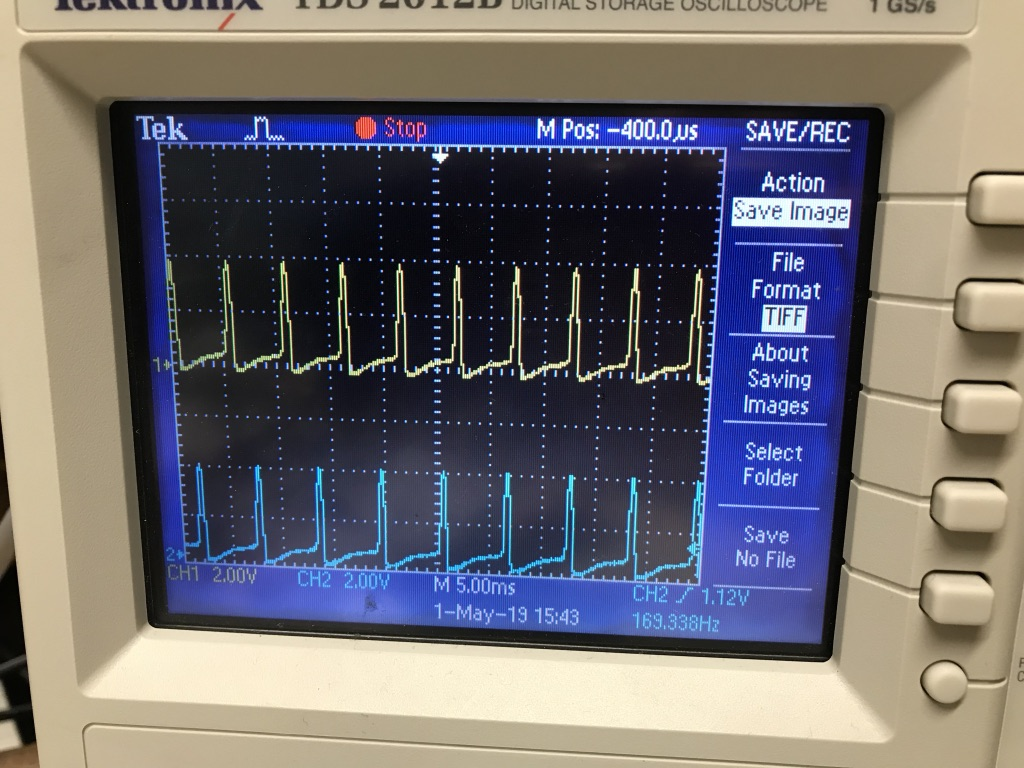
\includegraphics{pattern_generation}
\caption{The results of our pattern generation circuit was not found to be in correspondence with our theoretical analysis}
\end{figure}


\appendix

\chapter{Differential Equation Analysis}

\begin{figure}[h]
\centering
\begin{subfigure}{0.7\textwidth}
	\centering
	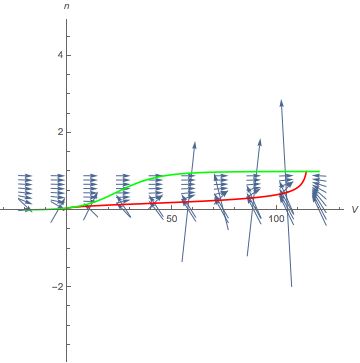
\includegraphics[width=0.7\textwidth]{fastFast_nullc.png}
	\caption{$I_{ext}=0$ nullclines}
\end{subfigure}
\begin{subfigure}{0.7\textwidth}
	\centering
	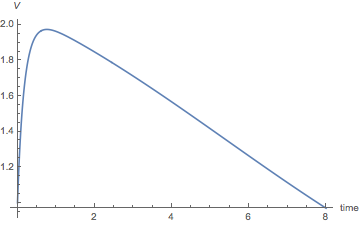
\includegraphics[width=0.7\textwidth]{fastFast.png}
	\caption{$I_{ext}=0$ action potential}
\end{subfigure}
	\caption{V-nullcline (Red) and n-nullcline (Green) for $I_{ext}$ on and off of simple constant $h$ model, with associated action potentials}
	\label{fig:first}
\end{figure}

In Figure \ref{fig:first}, we see the result of the Fitzhugh-Nagumo approximation. We can see that there are three potential intersections of the nullclines (two are present in the bottom left but difficult to visualize due to their close proximity), implying that there are excited and relaxed fixed points. If one looks closely at the vector field, the excited equilibrium (upper-right) appears to be attracting, and in the lower-left one equilibrium seems to be attracting while the other is a saddle. We'll call the one that is attracting in the lower-left the rest equilibrium, since it should correspond to the action potential going to rest. We also see that the action potential looks qualitatively different than it does in the unsimplified H-H model. The model seems less than ideal, but is a good initial step. 

We could treat $n$ and $h$ as bifurcation parameters. For example, we can use our physical intuition to consider the effects of increasing $n$ and decreasing $h$. Evidently, increasing $n$ corresponds to activation of K$^+$ conductance and deactivation of Na$^+$ conductance. As a result, we could predict the disappearance of the fixed point that corresponds to an excited state. Indeed, one can show that there is a saddle node bifurcation in this scenario resulting in the disappearance of the saddle and excited fixed points.\cite{keener}.

\bibliography{phy365.bib}
\bibliographystyle{plain}
\nocite{*}


\end{document}
nami